\documentclass[12pt]{report}

\usepackage{commands}
\usepackage{mathdots}

\begin{document}

\large

\begin{center}
 Math 586 Homework 3\\
 Due May 5\\
 By Marvyn Bailly (GitHub: MarvynB)\\
\end{center}

\normalsize

\hrule

%---------------%
%---Problem 1---%
%---------------%

%--status--$

\begin{problem}
    Consider solving the following heat equation with ``linked'' boundary conditions
  \begin{align*}
    \begin{cases}
        u_t = \frac 1 2 u_{xx}\\
        u(0,t) = s u(1,t)\\
        u_x(0,t) = u_x(1,t),\\
        u(x,0) = \eta(x),
    \end{cases}
    \end{align*}
    where $s \neq -1$.   Recall that the MOL discretization with the standard second-order stencil can be written as
    \begin{align*}
        U'(t) = -\frac{1}{2h^2} A U(t) + \begin{bmatrix} \frac{U_0(t)}{2h^2} \\ 0 \\ \vdots \\ 0 \\ \frac{U_{m+1}(t)}{2h^2} \end{bmatrix}, \quad A = \begin{bmatrix}
        2  & -1\\
        -1 & 2 & -1 \\
        & -1 & 2 & -1\\
        && \ddots & \ddots & \ddots \\
        &&& -1 & 2 \end{bmatrix}.
    \end{align*}
    The first boundary condition is naturally enforced via $U_0(t) = s U_{m+1}(t)$. Show that if we suppose
    \begin{align*}
        \frac{U_{1}(t) - U_0(t)}{h} = \frac{U_{m+1}(t) - U_m(t)}{h},
    \end{align*}
    then the MOL system becomes
    \begin{align}\label{mol}
        U'(t) = \frac{1}{2h^2} B U(t), \quad B = \begin{bmatrix}
        -2 + \frac{s}{1 + s} & 1 &&&& \frac{s}{1 + s}\\
        1 & -2 & 1 \\
        & 1 & -2 & 1 & \\
        &&\ddots & \ddots & \ddots \\
        &&&1 & -2 & 1 \\
        \frac{1}{1+s} &&&& 1 & -2 + \frac{1}{1+s} \end{bmatrix}.
    \end{align}
\end{problem}

\begin{solution}

  \noindent
  Consider the heat equation with "linked" boundary conditions
  \begin{align*}
    \begin{cases}
        u_t = \frac 1 2 u_{xx}\\
        u(0,t) = s u(1,t)\\
        u_x(0,t) = u_x(1,t),\\
        u(x,0) = \eta(x),
    \end{cases}
  \end{align*}
  where $s \neq -1$. We will use the method of lines discretization with the standard second-order stencil which can be written as
  \begin{align*}
    U'(t) = -\frac{1}{2h^2} A U(t) + \begin{bmatrix} \frac{U_0(t)}{2h^2} \\ 0 \\ \vdots \\ 0 \\ \frac{U_{m+1}(t)}{2h^2} \end{bmatrix}, \quad 
      A = \begin{bmatrix}
        2  & -1\\
        -1 & 2 & -1 \\
        & -1 & 2 & -1\\
        && \ddots & \ddots & \ddots \\
        &&& -1 & 2 \end{bmatrix}.
  \end{align*}
  The first boundary condition is naturally enforced via $U_0(t) = sU_{m+1}(t)$. Now if we suppose
  \begin{align*}
    \frac{U_{1}(t) - U_0(t)}{h} = \frac{U_{m+1}(t) - U_m(t)}{h},
  \end{align*}
  we can solve solve for $U_0$ and $U_{m+1}$ in terms of $U_1$ and $U_m$. Observe that
  \begin{align*}
    \frac{U_{1}(t) - U_0(t)}{h} &= \frac{U_{m+1}(t) - U_m(t)}{h}\\
    \iff U_1 - U_0 &= U_{m+1} - U_m\\
    \iff U_1 - U_0 &= \frac{U_0}{s} - U_m\\
    \iff  U_0 \paren{\frac{s+1}{s}} &= U_1 + U_m \\
    \iff  U_0 &= \paren{\frac{s}{s+1}}\paren{U_1 + U_m}.
  \end{align*}
  And similarly, we find that 
  \begin{align*}
    \frac{U_{1}(t) - U_0(t)}{h} &= \frac{U_{m+1}(t) - U_m(t)}{h}\\
    \iff U_1 - U_0 &= U_{m+1} - U_m\\
    \iff U_1 - sU_{m+1} &= U_{m+1} - U_m\\
    \iff U_{m+1} &= \paren{\frac{1}{s+t}}\paren{U_1 + U_m}.
  \end{align*}
  Thus when we apply the finite-centered difference of the form
  \[ 
    \frac{U_{j+1} - 2U_j + U_{j-1}}{h^2}
  \]
  we no longer need to use the boundary conditions on the edge cases $j=1,m$. For example when $j=1$ we have
  \[ 
    \frac{U_{2} - 2U_{1} + U_{0}}{h^2} = \frac{U_{2} - 2U_{1} + \paren{\frac{s}{s+1}}\paren{U_1 + U_m}}{h^2},
  \]
  and when $j=m$ we have
  \[ 
    \frac{U_{m+1} - 2U_m + U_{m-1}}{h^2} = \frac{\paren{\frac{1}{s+t}}\paren{U_1 + U_m} - 2U_m + U_{m-1}}{h^2}.
  \]
  Thus MOL discretization becomes
  \begin{align*}
    U'(t) = \frac{1}{2h^2} B U(t), \quad B = \begin{bmatrix}
    -2 + \frac{s}{1 + s} & 1 &&&& \frac{s}{1 + s}\\
    1 & -2 & 1 \\
    & 1 & -2 & 1 & \\
    &&\ddots & \ddots & \ddots \\
    &&&1 & -2 & 1 \\
    \frac{1}{1+s} &&&& 1 & -2 + \frac{1}{1+s} \end{bmatrix},
  \end{align*}
  where we also moved the minus sign into $B$.
\end{solution}

%----------------------------------------------------------------------------------------------------%
%\vskip 20pt
\newpage

%---------------%
%---Problem 2---%
%---------------%

%--status--$

\begin{problem}
    Apply the backward Euler method to \eqref{mol} to give
  \begin{align}\label{be}
    \left( I - \frac{k}{2h^2}B \right) U^{n+1} =  U^n, \quad U^n = \begin{bmatrix} U_1^n \\ U_2^n \\ \vdots \\U_m^n \end{bmatrix},
  \end{align}
  and write a routine to solve the system \eqref{mol} with the initial condition
  \begin{align*}
    \eta(x) = e^{-20(x-1/2)^2},
  \end{align*}
  using $k = h$ and $h = 0.001$ with $s = 2$.  Plot the solution at times $t = 0.001,0.01,0.1$.
\end{problem}

\begin{solution}

  \noindent
  Recall that the backward Euler method is defined by
  \[ 
    U^{n+1} = U^n + \frac{k}{2h^2} B U^{n+1}, \quad U^n = \begin{bmatrix} U_1^n \\ U_2^n \\ \vdots \\U_m^n \end{bmatrix}.
  \] 
  rearranging the terms we get
  \[ 
    U^{n+1}\left( I - \frac{k}{2h^2}B \right) = U^n.
  \]
  Now we wish to write a routine to solve \eqref{mol} with the initial condition
  \begin{align*}
    \eta(x) = e^{-20(x-1/2)^2},
  \end{align*}
  using $k = h$ and $h = 0.001$ with $s = 2$. To create the routine, I used Julia and implemented the Backward Euler method using the following code:
  \begin{python}
  function BE(m,uInit,T)
    h = 1/(m+1);
    k = h;
    s = 2;
    xs = (h:h:1-h)
    #create B
    B =  spzeros(m,m) + SymTridiagonal(fill(-2.0,m),fill(1.0,m-1));
    B[1,1] += s/(1+s);
    B[1,end] += s/(1+s);
    B[end,end] += 1/(1+s);
    B[end,1] += 1/(1+s);


    #BE
    u = uInit
    for i = k:k:T
        uNext = (I(m) - k/(2h^2) * B)\u
        u = uNext
    end
    return (u,xs)
  end
  \end{python}
  Running the backward Euler function for $t = 0.001,0.01,0.1$ and graphing the results, see Figure \ref{fig1}, we see that the solution behaves as expected as time evolves. 
  \begin{figure}[H]
    \centering
    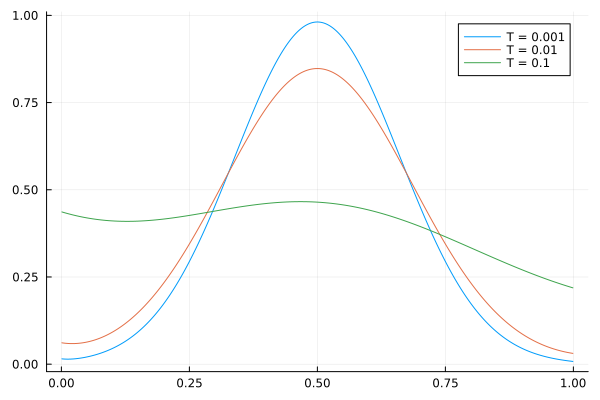
\includegraphics[width=0.5\textwidth,height=\textwidth,keepaspectratio]{images/2.png}
    \caption{Backward Euler Solution to equation \eqref{mol} at different times. Blue is the solution at $t=0.001$, orange at $t=0.01$, and green at $t=0.1$.}
    \label{fig1}
  \end{figure}

\end{solution}

%----------------------------------------------------------------------------------------------------%
%\vskip 20pt
\newpage

%---------------%
%---Problem 3---%
%---------------%

%--status--$

\begin{problem}
    In the next two problems, you will use the heat equation to assist with a statistics problem.
  \begin{itemize}  
\item Consider data points $X_1,X_2,\ldots,X_N,\ldots$ each being a real number arising from a repeated experiment.  We may want to know what probability distribution (if any) they come from.  One way of coming up with an approximation to the density is to use
  \begin{align}\label{eq:heat-evolve}
    \frac{1}{N} \sum_{j=1}^N \frac{1}{\sqrt{2 \pi t}} \exp \left( - \frac{(x - X_j)^2}{2t} \right), \quad t > 0.
  \end{align}
  Use normally distributed random data ({\tt X = randn(n)} in {\tt Julia},  {\tt X = randn(n,1)} in {\tt Matlab} and {\tt X = numpy.random.randn(n,1)} in {\tt Python}) with $n = 10000$ and plot this function for $t = 0.001,0.01,0.1,1,10$ and compare it with the true probabilty density function for the data:  $\rho(x) = \frac{1}{\sqrt{2 \pi}} e^{-x^2/2}$. Visually, which ``time'' $t$ gives the best approximation?\\

  \underline{Note}:  The solution of the heat equation $u_t = \frac 1 2 u_{xx}$ with initial condition $u(x,0) = \delta(x)$ where $\delta$ is the standard Dirac delta function is given by $u(x,t) = \frac{1}{\sqrt{2 \pi t}} \exp \left( - \frac{x^2}{2t} \right)$.  So \eqref{eq:heat-evolve} can be seen as the solution of $u_t = \frac 1 2 u_{xx}$ with
  \begin{align*}
    u(x,0) = \frac{1}{N} \sum_{j=1}^N \delta(x-X_j).
  \end{align*}

\item The previous approach works well if the underlying distribution is smooth and decays exponentially in both directions.  But there are physical situations within cell biology, in particular, where the density should only be non-zero on a finite interval $[0,1]$ and satisfy some natural boundary conditions:
  \begin{align*}
    \rho(0) = s \rho(1), \quad \rho'(0) = \rho'(1).
  \end{align*}
  An example of such a function for $s = 2$ is given by
  \begin{align*}
    \rho(x) = - \frac 2 3 x + \frac 4 3 + \frac 1 2 \sin(2 \pi x).
  \end{align*}
  Code to generate $X_1,X_2,\ldots,X_N,\ldots$ with this probability density in our three languages is given at the end of the homework.  Repeat the calculation in the previous part with this data, $X_1,X_2,\ldots$.
    
\end{itemize}
\end{problem}

\begin{solution}

    \noindent
    we wish to create a routine to approximate the density of normally distributed data points using equation \ref{eq:heat-evolve}. To achieve this, I will use Julia, where \verb+randn(n)+ is used to generate $n$ normally distributed random data points. We will use $n=10000$. I implemented \ref{eq:heat-evolve} and the true solution and their plotting in Julia with the following code:
    \begin{python}
      getTrueDensity = (x) -> 1/(sqrt(2 * pi))*exp(-x^2/2)
      getApprox = (n,xs,t,points) -> map(xs -> sum(point -> begin (1/n)*(1/(sqrt(2*pi*t)))*exp(-(xs - point)^2/(2t)) end, points), xs)

      n = 10000;
      points = randn(n);
      xs = -3:0.01:3;
      ts = [0.001,0.01,0.1,1,10]; 

      graph = plot(xs,map(getTrueDensity,xs),xlabel="X's",ylabel="Density",label="True Solution");
      for i=1:length(ts)
          graph = plot!(xs,getApprox(n,xs,ts[i],points),label="t = "*string(ts[i]));
      end
    \end{python}
    Plotting the solutions with $t = 0.001,0.01,0.1,1,10$ compared to the true solution, as seen in figure \ref{fig2}, we see that $t=0.01$ gives the best approximation.

    \begin{figure}[H]
      \begin{subfigure}[b]{0.5\linewidth}
        \centering
        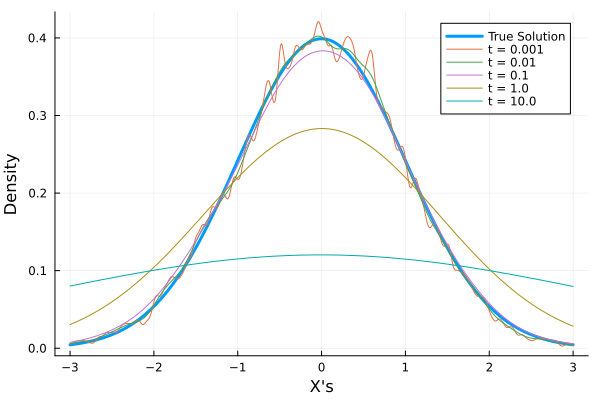
\includegraphics[width=\linewidth]{images/3a1.png}
        \caption{}
        \label{fig2:a}
        \vspace{4ex}
      \end{subfigure}%%
      \begin{subfigure}[b]{0.5\linewidth}
        \centering
        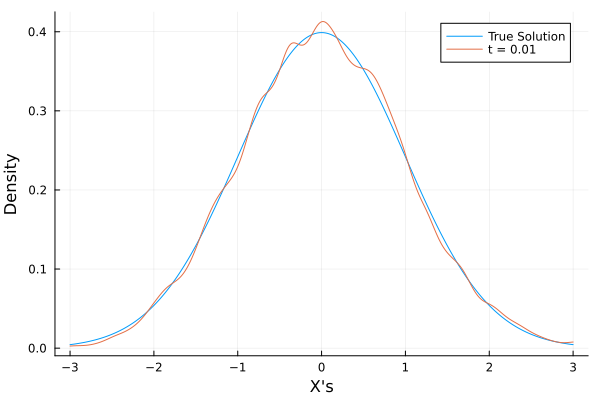
\includegraphics[width=\linewidth]{images/3a2.png}
        \caption{}
        \label{fig2:b}
        \vspace{4ex}
      \end{subfigure}
      \caption{Plotting solution from \ref{eq:heat-evolve} compared to the true solution of normally distributed data. In (a), we compared the true solution with $t=0.001,0.01,0.1,1,10$ while in (b) we see that $t=0.01$ gives the closest approximation to the true solution.}
      \label{fig2}
  \end{figure} 


    \noindent
    We repeat the process but now using data points sampled from \verb+prand+ which has distribution of the form
    \begin{equation}\label{weirdDataPoints}
      \rho(x) = -\frac{2x}{3} + \frac{4}{3} + \frac{1}{2}\sin(2\pi x).
    \end{equation}
    Plotting the approximate solutions for $t = 0.001,0.01,0.1,1,10$ compared to the true solution, as seen in figure \ref{fig3}, we see that $t=0.001$ now best approximates the true solution.
    

    \begin{figure}[H]
      \begin{subfigure}[b]{0.5\linewidth}
        \centering
        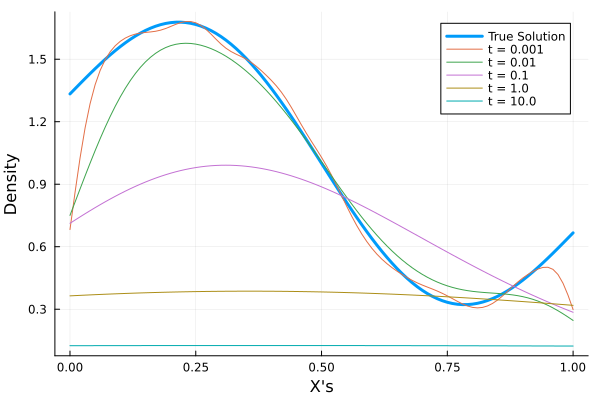
\includegraphics[width=\linewidth]{images/3b1.png}
        \caption{}
        \label{fig3:a}
        \vspace{4ex}
      \end{subfigure}%%
      \begin{subfigure}[b]{0.5\linewidth}
        \centering
        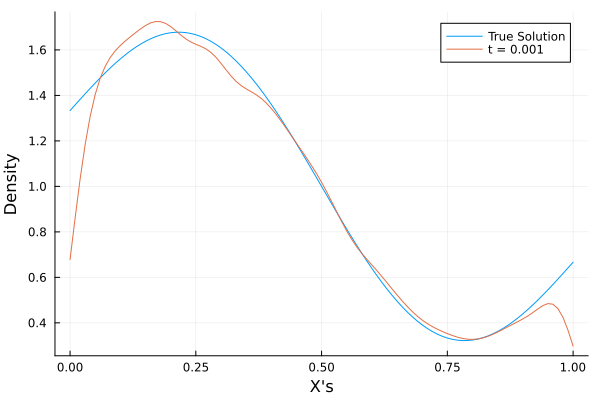
\includegraphics[width=\linewidth]{images/3b2.png}
        \caption{}
        \label{fig3:b}
        \vspace{4ex}
      \end{subfigure}
      \caption{Plotting solution from \ref{eq:heat-evolve} compared to the true solution where the data is generated from prand. In (a), we compared the true solution with $t=0.001,0.01,0.1,1,10$ while in (b) we see that $t=0.001$ gives the closest approximation to the true solution.}
      \label{fig3}
  \end{figure}

  \begin{python}
  function prand(m)
    p = x -> -(2.0/3)* x .+ 4.0/3 .+ .5*sin.(2* pi * x )
    B = 1.7
    out = fill(0.,m)
        for j = 1: m
            u = 10.
            y = 0.
            while u >= p(y)/ B
                y = rand()
                u = rand()
            end
        out[j] = y
    end
    return out
  end
  \end{python}


\end{solution}

%----------------------------------------------------------------------------------------------------%
%\vskip 20pt
\newpage

%---------------%
%---Problem 4---%
%---------------%

%--status--$

\begin{problem}
    Consider binning data $X_1,X_2,\ldots,X_N$, $X_j \in (0,1)$ as follows:
  \begin{itemize}
  \item Find $Y_i$ so that $Y_i$ is the number of data points $X_j$ that lie in the interval $[ih,(i+1)h) = [x_i,x_{i+1})$.
  \item Set $U_i^0 = \frac{Y_i}{h N}$.
  \end{itemize}
  With $N = m$, $h = 0.0001$, $k = 10h$, $s = 2$, generate $X_1,\ldots,X_N$ using the {\tt prand} function, and bin the data to get the initial condition $U_i^0$, $i = 1,2,\ldots,m$ for the MOL discretization \eqref{mol}.  Solve with this initial condition using your code from {\textbf{Problem 2}} to times $t = 0.001,0.01,0.1$.  Compare this with Part 2 of Problem 3.
\end{problem}

\begin{solution}

    \noindent
    We now wish to use the Backward Euler method we implement in Problem 2 to approximate the distribution of the \verb+prand+ function. We will use the same code from Problem 2 with $N=m, h=0.0001, k=10h, \and s=2$. Next, we generate $X_1, \dots, X_N$ data points using the \verb+prand+ function and bin the data as described in the problem statement. We used the following Julia code to bin our data:
    \begin{python}
    function binData(data)
      Y = zeros(length(data))
      for i=1:length(data)
          for j=1:m
              if data[i] >= j*h && data[i] < (j +1)*h
                  Y[j] += 1
              end
          end
      end
      uInit = Y./(h*m)
      return uInit
    end
    \end{python}
    We now run Backward Euler with the new initial condition for times $t=0.001,0.01,0.1$ and compare them to the true solution given by Equation \ref{weirdDataPoints}. Observing the graph, seen in Figure \ref{fig4}, we see that the solutions are similar to those seen in Figure \ref{fig3:a} expect the Backward Euler method handles the boundary condition at $x=1$ significantly better than equation \ref{eq:heat-evolve}.



  \begin{figure}[H]
    \centering
    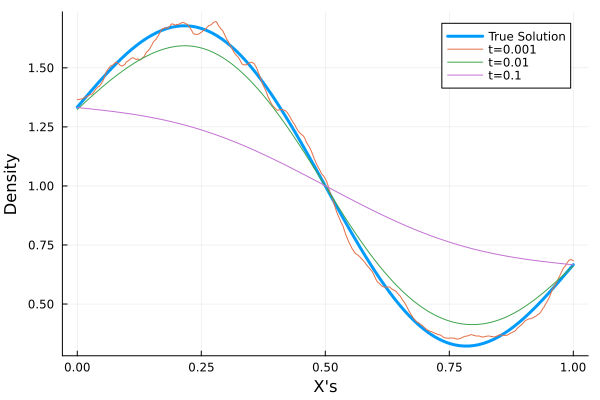
\includegraphics[width=0.75\textwidth,height=\textwidth,keepaspectratio]{images/4.png}
    \caption{Backward Euler in conjugation with binning is used to approximate the distribution of data generated from prand. The true solution shown in blue is graphed from \ref{weirdDataPoints}.}
    \label{fig4}
  \end{figure}
\end{solution}

%----------------------------------------------------------------------------------------------------%
%\vskip 20pt
\newpage

%---------------%
%---Problem 5---%
%---------------%

%--status--$

\begin{problem}
    Suppose the following is true: For $s > 0$, if $y$ is a vector with non-negative entries and $\left( I - \frac{k}{2h^2}B \right) x = y$ then $x$ has non-negative entries. \\

  
      \noindent For $s > 0$, establish the following:
       \begin{itemize}
       \item $\begin{bmatrix} 1 & 1 & \cdots & 1 \end{bmatrix} B = 0$ and therefore $\sum_j U_j^n = \sum_j U_j^0$ for all $n$.
         \item  Show that \eqref{be} is Lax-Richtmyer stable in the $1$-norm, $\|u\|_1 = h \sum_{i=1}^m |u_i|$.
    \end{itemize}
\end{problem}

\begin{solution}

    \noindent
    Let $s > 0$. We assume that if $y$ has non-negative entries and $(I - \frac{k}{2h^2}B)x = y$ (same $B$ from Equation \ref{mol}), then $x$ has non-negative entries. We first wish to show  that $\begin{bmatrix} 1 & 1 & \cdots & 1 \end{bmatrix} B = 0$. Observe that 
    \[ 
      \paren{\begin{bmatrix} 1 & 1 & \cdots & 1 \end{bmatrix} B}_1 = -2 + \frac{s}{1+s }+ 1 + \frac{1}{1 + s} = -1 + \frac{s}{1+s}+\frac{1}{1+s} = 0,
    \]
    and 
    \[ 
      \paren{\begin{bmatrix} 1 & 1 & \cdots & 1 \end{bmatrix} B}_m = \frac{s}{1+s} + 1 - 2 + \frac{1}{1+s} = -1 + 1 = 0,
    \]
    and 
    \[ 
      \paren{\begin{bmatrix} 1 & 1 & \cdots & 1 \end{bmatrix} B}_j = -2 + 1 + 1 = 0,
    \]
    for $1< j < m$. Thus we have that 
    \[ 
      \begin{bmatrix} 1 & 1 & \cdots & 1 \end{bmatrix} B = 0.
    \]
    To show $\sum_j U_j^n = \sum_j U_j^0$, note that using $\begin{bmatrix} 1 & 1 & \cdots & 1 \end{bmatrix} B = 0$ we have
    \[ 
      \begin{bmatrix} 1 & 1 & \cdots & 1 \end{bmatrix}(I - \frac{k}{2h^2}B) = \begin{bmatrix} 1 & 1 & \cdots & 1 \end{bmatrix} - \frac{k}{2h^2} \begin{bmatrix} 1 & 1 & \cdots & 1 \end{bmatrix} B = \begin{bmatrix} 1 & 1 & \cdots & 1 \end{bmatrix}.
    \]
    Since $(I - \frac{k}{2h^2}B) U^{n+1} = U^{n}$, for $n=0,1,2,\dots$, inductively we get that 
    \[
      \paren{I - \frac{k}{2h^2}B}^nU^n = U^0, \quad \forall n.
    \]
    Observe that multiplying both sides by $\begin{bmatrix} 1 & 1 & \cdots & 1 \end{bmatrix}$ yields
    \begin{align*}
      \begin{bmatrix} 1 & 1 & \cdots & 1 \end{bmatrix} \cdot U^0 &= \begin{bmatrix} 1 & 1 & \cdots & 1 \end{bmatrix} \cdot \paren{I - \frac{k}{2h^2}B}^n U^n \\
      &= \paren{\begin{bmatrix} 1 & 1 & \cdots & 1 \end{bmatrix} \paren{I - \frac{k}{2h^2}B}}\cdot \paren{I - \frac{k}{2h^2}B}^{n-1}U^n\\
      &= \begin{bmatrix} 1 & 1 & \cdots & 1 \end{bmatrix} \cdot \paren{I - \frac{k}{2h^2}B}^{n-1}U^n\\
      &\vdots\\
      &= \begin{bmatrix} 1 & 1 & \cdots & 1 \end{bmatrix} \cdot \paren{I - \frac{k}{2h^2}B}U^n\\
      &= \begin{bmatrix} 1 & 1 & \cdots & 1 \end{bmatrix} \cdot U^n.
    \end{align*}
    Therefore we have shown that
    \[ 
      \begin{bmatrix} 1 & 1 & \cdots & 1 \end{bmatrix} \cdot U^0 = \begin{bmatrix} 1 & 1 & \cdots & 1 \end{bmatrix} \cdot U^n \implies \sum_j U_j^0 = \sum_j U_j^n.
    \]
    Next we wish to show that equation \ref{be} is Lax-Richtmyer stable in the $1-$norm. Recall that Lax-Richtmyer stability is defined as
    \[ 
      \left\| \paren{I - \frac{k}{2h^2}B}^{-n} \right\|_1 \leq c_T,
    \]
    where $c_T > 0$. Let's begin by showing that $\paren{I - \frac{k}{2h^2}B}$ is invertible by showing that the kernel is trivial. Let $x$ be in the null space of $\paren{I - \frac{k}{2h^2}B}$, then by definition
    \[ 
      \paren{I - \frac{k}{2h^2}B} x = 0,
    \]
    and since $0$ has nonzero entries, we also know $x$ has nonzero entries by our first assumption. Next multiplying both sides by $\begin{bmatrix} 1 & 1 & \cdots & 1 \end{bmatrix}$ yields 
    \begin{align*}
      0 &= \begin{bmatrix} 1 & 1 & \cdots & 1 \end{bmatrix} \paren{I - \frac{k}{2h^2}B} x\\ 
      &= \begin{bmatrix} 1 & 1 & \cdots & 1 \end{bmatrix} I x - \begin{bmatrix} 1 & 1 & \cdots & 1 \end{bmatrix} Bx \\
      &= \begin{bmatrix} 1 & 1 & \cdots & 1 \end{bmatrix} x\\
      &= \sum_j x_j,
    \end{align*}
    and since $x_j > 0$ for all $j$ and $\sum_j x_j = 0$, then $x_j = 0$ for all $j$. Thus the kernel is trivial and the inverse exists. Let $A = \paren{I - \frac{k}{2h^2}B}^{-1}.$ Then observe that for an arbitiary $u^0$ we have 
    \begin{align*}
      \| A^n u^0 \|_1 &= \|A^n \sum_j u_j^0 e_j\|_1\\
        &\leq \sum_j \| A^n u_j^0 e_j \|_1\\
        &= h \sum_j|u^0_j|\sum_i(|A^n e_j|)_i,\\
    \end{align*} 
    where $e_j$ has zeros in all entries expect for $j$th entry being one. Thus $e_j$ has nonnegative entries. Since $\sum_i(A^n u^0)_i = \sum_i(u^n)_i = \sum_i (u^0)_i$, letting $e_j = u^0$ gives that $\sum_i(|A^n e_j|)_i = \sum_i(|e_j|)_i = 1$ for all $j$. Thus we have that
    \begin{align*}
      \| A^n u^0 \|_1 \leq h \sum_j|u^0_j|\sum_i(|Ae_j|)_i &= h \sum_j|u^0_j| = \| u^0 \|_1.
    \end{align*}
    This implies that
    \[ 
    \| A^n \|_1 \leq \frac{\| A^n u^0 \|_1}{\| u^0 \|_1} \leq 1,  
    \]
    therefore if we let $c_T = 1$ we have that
    \[ 
      \|A^n\|_1 < c_T
    \]
    and thus equation \ref{be} is L-R stable.


\end{solution}

%----------------------------------------------------------------------------------------------------%
%\vskip 20pt
\newpage

%---------------%
%---Problem 6---%
%---------------%

%--status--$

\begin{problem}
    Consider the bi-infinite matrix
    \begin{align*}
      L = \begin{bmatrix}
        \ddots & \vdots & \vdots & \vdots  & \iddots \\
        \cdots & L_{-1,-1} & L_{-1,0} & L_{-1,1} & \cdots \\
        \cdots & L_{0,-1} & L_{0,0} & L_{0,1} & \cdots \\
        \cdots & L_{1,-1} & L_{1,0} & L_{1,1} & \cdots \\
        \iddots & \vdots & \vdots & \vdots & \ddots
      \end{bmatrix}.                
    \end{align*}
    Suppose the matrix $L$ defines a bounded linear operator on $\ell^2(\mathbb Z)$ via matrix-vector multiplication with
    \begin{align*}
     \ell^2(\mathbb Z) \ni V = \begin{bmatrix} \vdots \\ V_{-1} \\ V_0 \\ V_1 \\\vdots \end{bmatrix}.
    \end{align*}
    Show that $L$ is translation invariant if and only if $L_{i,j} = c_{i - j}$ for a sequence $(c_j)_{j=-\infty}^\infty$, i.e., $L$ is a Toeplitz matrix.  Hint: Apply $L$ to the standard basis vectors.
\end{problem}

\begin{solution}

    \noindent
    Consider the bi-infinite matrix
    \[ 
      L = \begin{bmatrix}
        \ddots & \vdots & \vdots & \vdots  & \iddots \\
        \cdots & L_{-1,-1} & L_{-1,0} & L_{-1,1} & \cdots \\
        \cdots & L_{0,-1} & L_{0,0} & L_{0,1} & \cdots \\
        \cdots & L_{1,-1} & L_{1,0} & L_{1,1} & \cdots \\
        \iddots & \vdots & \vdots & \vdots & \ddots
      \end{bmatrix}.
    \]
    Suppose the matrix $L$ defines a bounded linear operator on $\ell^2(\mathbb Z)$ via matrix-vector multiplication with
    \begin{align*}
     \ell^2(\mathbb Z) \ni V = \begin{bmatrix} \vdots \\ V_{-1} \\ V_0 \\ V_1 \\\vdots \end{bmatrix}.
    \end{align*}
    Let $e_j$ be the standard basis vector where the $j$th element is one and all others are zero and let $(L)_k$ denote the $k$th row of $L$. Then
    \[ 
      (Le_j)_i = (L_j)_i = L_{i,j}.
    \]
    Now consider the shift operator $S_l$ where $l \in \Z$. Then $S_l e_j = e_{j+l}$ and note that due to the construction of $L$, $(S_{-l}L)_i = (L)_{i+l}$. Then we have
    \begin{align*}
      (S_{-l}LS_le_j)_i = (LS_le_j)_{i+l} = (Le_{j+l})_{i+l} = L_{i+l,j+l}. 
    \end{align*}
    Since the $e_j$'s form a basis for $\ell^2(\mathbb Z)$, any $V \in \ell^2(\Z)$ can be decomposed into a sum of $e_j$'s. Thus we have that 
    \[ 
      LV = (S_{-l}LS_{l})V \iff L_{i,j} = L_{i+l,j+l}. 
    \]  
    Therefore $L$ is shift-invariant if and only if $L_{i,j} = L_{i+l,j+l}$ which is the definition of a Toeplitz matrix, i.e. $L_{i,j} = c_{i-j}$ for a sequence $(c_j)^\infty_{j=-\infty}$.



\end{solution}

%----------------------------------------------------------------------------------------------------%
%\vskip 20pt
\newpage

%---------------%
%---Problem 7---%
%---------------%

%--status--$

\begin{problem}
    A challenge (extra credit, total score cannot exceed 20):  In the notation of Problem 2, for $s > 0$, establish:
  \begin{itemize}
  \item If $y$ is a vector with non-negative entries and $\left( I - \frac{k}{2h^2}B \right) x = y$ then $x$ has non-negative entries.
  \end{itemize}
  Note that this shows that if $\sum_j U_j^0 =1$ then at each step $n$ we can interpret $U_j^n$ as the evolution of a probability distribution.
\end{problem}

\begin{solution}
    \noindent
    This is a solution
\end{solution}

%----------------------------------------------------------------------------------------------------%
%\vskip 20pt
\newpage


\end{document}